\documentclass{article}
\usepackage{csvsimple}
\usepackage{amsmath}
\usepackage{amssymb}
\usepackage{graphicx}

\begin{document}

%insert your content here..

\section{Student content}


 \subsection{Constance Hendrix}
Greetings.  My name is Constance Hendrix.  I go-by Constance.  I’m a wife, an electrical engineer, a 30-year Air Force veteran, and a current Engineering Security PhD student here at UCCS (see Canvas picture in Figure 1. 
\begin{figure}[h]
    \centering
    
\includegraphics[scale=0.06]{hendrix_canvas.jpg}
    \label{fig:me}
    \caption{Constance, about to be fed, while on a overdue retreat!}
\end{figure}
I’m coming in with a Masters of Science degree in electrical engineering with a focus in navigation systems from the Air Force Institute of Technology and a Masters of Business Administration from the University of West Florida.  I'm also a licensed electrical engineer in the state of Colorado and a certified Project Management Professional. My overarching goal for graduate school is to make a significant contribution to my engineering field and lay the foundation for a future in academia.  My research interests include reliable and accurate navigation, secure satellite communications, biologically-influenced design, artificial intelligence, and signal processing.  I have yet to specifically identify my security research topic, but know it will include artificial intelligence, signal processing, and/or edge computing. I hope to select a topic by next semester and will be preparing for my oral qualifier next Spring as well.  My goal for this course is to narrow my research focus for my degree, learn new and efficient ways to conduct research, and develop research questions. Outside of school, I work part-time as a position, navigation and timing (PNT) engineer, enjoy reading, working on stained glass creations, quilting, camping, fly fishing, hiking, cooking, and gardening.  Quilting is a tradition for the women in my family.  Even though I just recently started, I am excited to carry on this tradition.

\textbf{Question from Jackie}
Hi Constance, you have a very impressive knowledge background. I do not know a lot about navigation systems, but I always have a question on how navigation works when two teams are digging an undersea tunnel toward each other and they align perfectly?

\textbf{Question from Jordan}
Have you used git before? Most EEs I know end up in software at some point. I've only used Subversion before this year so git is still new to me.



 \title{Third Week's Git Assignment} 

 \maketitle


\begin{abstract}
This document provide a brief introduction to Maximus' personal life, his goals, and his love for privacy.
\end{abstract}
\section{Background and Objectives for This Course}
Maximus a.k.a. \emph{"Cyber Gladiator"} works in the field of cybersecurity and is currently studying security this semester to focus on CPS/IoT designs, vulnerabilities, and flaws. As a student, he loves/ obsessed with privacy, and he hopes that he will become a more effective computer science researcher focusing on CPS/IoT systems by taking computer science research course this Fall.

Maximus' main area of interest includes (but not limited to) information systems’ vulnerabilities, vulnerabilities in system design and implementations, cyber risk assessment of IoT systems, and management of the risk in critical information systems in the broader context of their daily effects on individuals.


\begin{figure}[htbp]
\centerline{
\includegraphics{a481.jpg}}
\caption{Maximus is currently looking at the mirror.}
\label{fig}
\end{figure}

\subsection{James Bond(Peng)}
Before I study in UCCS, I was security solution architect and software engineer. I worked for Newegg, and Hewlett-Packard. I developed security for BIOS (basic input output system) and firmware in laptops, developed infrastructure security for fraud detection systems and search systems in E-Commerce. I also served in military, for cyber operation and radar systems for Coast Guard. I studied electrical engineering and energy systems in undergraduate and high school.

My recent research interest now is signal intelligence (SIGINT), and advanced persistent threats (APTs) in embedded systems. Fields I've done are: 

\begin{itemize}
\item adversarial machine learning (artificial intelligence, intrusion detection and operation systems)
\item lightweight provenance (operating systems)
\item trust execution and zero trust architecture (cloud, privacy and cryptography)
\item fuzzing for satellite embedded systems (vulnerability scanning, protocol state machine, flight software)
\end{itemize}

I like not only coding, reading but also sports. I did fencing in elementary school and, after high school, Greco-Roman wrestling, boxing, cage fight, and surfing (both long board and short board). Now in the mountains of Colorado Springs, I swim instead. I am glad to learn from you guys. 

\begin{figure}[h]
  \centering
  
\includegraphics[width=180pt]{flainggg.jpg}
  \caption{Profile Picture on Office360}
  \label{fig.q1a}
\end{figure}

\textbf{Question for James Peng from Constance Hendrix}:  Hi again, James.  I saw you served in the Coast Guard as a Cyber Operator -- very exciting!  Where have you been stationed?
\textbf{Question for James Peng from Lori Babyak}:  Hi James. Thanks for fixing my problems in Babyak.txt - I appreciate it!  You've done some interesting work - I hope you can explain it to me sometime.

%
%\usepackage{tabularx} % extra features for tabular environment
%\usepackage{amsmath}  % improve math presentation
%\usepackage{graphicx} % takes care of graphic including machinery
%\usepackage[margin=1in,letterpaper]{geometry} % decreases margins
%\usepackage[utf8]{inputenc}
%%\usepackage{cite} % takes care of citations
%\usepackage[USenglish]{babel}
%\usepackage[utf8]{inputenc}
%
%\usepackage[backend=biber]{biblatex}
%\usepackage{csquotes}

%
%
%
%\usepackage[final]{hyperref} % adds hyper links inside the generated pdf file
%\hypersetup{
%	colorlinks=true,       % false: boxed links; true: colored links
%	linkcolor=blue,        % color of internal links
%	citecolor=blue,        % color of links to bibliography
%	filecolor=magenta,     % color of file links
%	urlcolor=blue         
%}
%

%++++++++++++++++++++++++++++++++++++++++


%\begin{document}

\title{Git Assignment - CS 6000}
\author{L. Babyak}
\date{September 15, 2020}
\maketitle

\section{Section 1}

My name is Lori Babyak.  I am a first year Computer Science PhD student at the University of Colorado, Colorado Springs. I hold a Bachelor's Degree in Computer Science from UT Austin and a Master's degree, also in Computer Science, from Texas State University. My goals for this course - CS 6000 Computer Science Research Methods- are to learn to research, read, and eventually produce research papers on subjects of interest in Computer Science. Additionally, I am looking forward to getting to know other students in the class and work collaboratively towards goals. Something personal about myself is that I have three grown children, two of whom live in the Denver area. Also, I took an extended vacation with a couple of friends in August. We visited Colorado Springs, Wyoming and South Dakota. In South Dakota, we visited Mt. Rushmore, the Crazy Horse Sculpture, and Custer State Park - where we saw free-roaming bison in their natural environment. I am happy and excited to be part of the UCCS community, and my hope is to make significant contributions to the field.

\begin{figure} [h!]
    \centering
    
\includegraphics[width=.4\textwidth]{LoriSDSmall.JPG} 
    \caption{A photo of Lori Babyak in front of Crazy Horse sculpture, outside Custer, SD, August 2020}
\end{figure}


\textbf{Question  to Lori Babyak from Constance Hendrix}:  I traveled to Wyoming and South Dakota in July.  Did you have the chance to see Devils Tower?

\textbf{Answer to Question from Constance Hendrix}: We drove through Wyoming and stopped in Torrington.  We only had a couple of days in SD, so we visited Mt. Rushmore, the Crazy Horse Sculpture and Custer State Park.  I don't think we saw Devil's Tower. There's so much to see there!

\textbf{Question from Jackie}
Hi Lori, thanks for sharing. I went to those places twice. The first time was in 2013, and the second time was in 2018. To be honest, I did not see much progress on the Crazy Horse. My questions would be: since you are in Colorado Springs, are you going to snow ski? If you already did, how much you enjoy the mountain views at the top? the cog train is a fun ride, too. 

\textbf{Answer to Jackie from Lori Babyak}: Hi Jackie, I guess I never mentioned that I actually live in Austin, Texas and am doing everything remote this semester! As far as skiing, I have not skied in CO Springs.  I have skied Keystone, Breckenridge, Copper Mountain, Vail and Park City, Utah. I am not an expert by any means, and I mostly enjoy the outdoors on the trips. I took the train to the top of Pike's Peak, and the views are amazing (but, it's very cold up there).  I think my favorite mountain top view was in SW Colorado, in the four-corners area, where I got a view of 4 states at once - maybe it was in Mesa Verde? Anyway, I really enjoy travelling and CO!


\section{Something About Me}
I am a first year PhD student in the UCCS. I am a photographer in my leisure time. I started this hobby from 2012. Throughout the past few years, I have helped friends recording the moments for their wedding, graduation parties, newborn baby, housewarming party, Halloween party, etc. When I travel, I enjoy capturing the beautiful nature. Beyond this, I like to disassemble and reassemble things then make improvements that fit my needs. If the product does not exist, I create my own. I sometimes play games with friends; this is a way of getting out of the busy life and relaxing and rebounding with friends. Snow ski and water ski are the two sports I enjoy. One is for winter and the other for summer. Here is a picture of me taken by myself.

\begin{figure}[htbp]
\centerline{
\includegraphics{zhang.jpg}}
\caption{Portrait of Kelei Zhang}
\label{fig}
\end{figure}

Question from Jordan: When I first read this, I missed the bit about you being a photographer. I was confused because it seemed like grad school was a hobby from 2012! :) What is the coolest picture you have taken?
Hi Jordan, thanks for asking the question. I think one of the coolest pictures I had taken was the Big Boy Steam Train. 2019 was the 150th anniversary of Big Boy on the railway. and it was snowing on the day I took the picture. With the team engine and the snowy day, it was quite a beautiful and unforgettable scene. 

Question for Zhang from James Peng: Hi, Zhang, that's awesome to obtain an ability of photography. I'd like to know how you guys capture or design the "composition" of certain moment? For example, in like 3 seconds, you need to decide what moment and how much and what things should be in your frame. This is amazing. How do you guys improve your decision making on the matter? 
Hi James, this is a very good question. I think the most important thing to take a good picture is to learn your camera and master the basic operation. Photography is split into different fields: portraiture, landscape, event, studio, action, etc. I think your question is more about event and action/sports photography where the person has to capture the subject very quickly and also compose perfectly. Well, that almost never happens. For these situations, either the photographer take a series of pictures to capture then select the best one, or they pre compose and wait for the moment. Sometimes, they sit still hours after hours, just like snipers. When they have a clear image, they usually crop to make a better composition. 


%%%%%%%%%%%%%%%%%%%%%%%%%%%%%%%%%%%%%%%%%%%%%%%%%%%%
%    Jordan Scott    %
%%%%%%%%%%%%%%%%%%%%%%%%%%%%%%%%%%%%%%%%%%%%%%%%%%%%
%\documentclass{article}

%\usepackage[utf8]{inputenc}
%\usepackage[english]{babel}
%\usepackage{graphicx}


%\begin{document}
	
	%\title{CS6000 Journal}
	%\author{Jordan Scott} 
	%\maketitle
	
	\section{\textbf{CS6000 Journal - Jordan Scott}}
	
	
	\begin{figure}
		\centering
		
\includegraphics[width=0.4\linewidth]{jordan.jpg}
		\caption{Jordan Scott}
	\end{figure}

	\paragraph*{Contact Info: } jscott21@uccs.edu \\
	https://www.linkedin.com/in/jordan-cancer-scott/\\
	https://github.com/jordanmscott/uccs


	\paragraph*{About Me}
		
		
		
	I am just starting my PhD in Security program. My goal for this course is to get into a research frame of mind, learn the modern tricks and tips, and help refine my dissertation topic.
	
	
	I am really interested in learning more about zotero and latex. I gained some experience with zotero last year, but previously I've only been aware of manual tracking and editing. It's nice to know that technology has evolved quite a bit with research and data management.
	

	I have done stand-up comedy twice. My set was mostly cybersecurity related and I received a number of laughs. I'm not sure if my comedy career will continue, but my career will definitely be full of comedy. 
	

	
	
	
	\paragraph*{\textbf{Questions}}
	
	Question and Answers
	
	
	Question 1 - Hi Jordan, I am just beginning my PhD program this year also!  I am learning a lot, trying to wrap my head around many things.  Dr. Kalita is my faculty advisor and I am studying AI.  I don't have a definite plan of study yet.  I'm learning so many things from this class about research. Another learning curve.  I don't know about you, but I am spending endless hours figuring out LaTex and github. I'll get there, though.  What are your impressions so far?
	
	
	Answer 1 - I like how the research methodologies have used software best practices to advance. The learning curve definitely exists though. I think this class has done a great job in getting us on the same page and moving towards using the tools properly. I suspect it will be a huge help later down the line when we are in a hundred page documument with hundreds of references.

	
	Question 2 - Question for Jordan Scott from James Peng: Hi, Jordan, I would like to ask you what is the most challenging experience/ things when you are  in comedy industry? I always feel you guys are awesome, like "positive/ joy-sharing version of lawyers", very good at public speaking, rhetoric, and know very well with the "jury".
	
	
	Answer 2 - Comedy is some awkward balance of saying what is on your mind, taking risk regardless of opinions, timing, and getting people into a mood. I think it probably has some of the same science behind it as music. Instead of beats per minute, its laughs per joke. My biggest challenge is memory though. I have a hard time remembering a script so I do more reading than natural delivery like the pros. I can talk and just keep going without a script, but the timing and order of things matter enough to where scripts have advantages. I think that's something I will just have to keep working on.


	\paragraph*{\textbf{Merge Conflict Notes:}}
	
	
	Not having access to the project seemed frustrating and took a bit to even figure out that was the problem. For my setup, I chose to use TeXstudio on a virtual box. The git clone part was easy. Getting the Assignment3 file to build was not. There were dependencies I needed to download/install into TeXstudio which was a challenge in itself, all related to the csvsimple function. Eventually got all that working. Then trying to figure out git itself... Got the commit part, the pull, the merge (had to install and configure a compare tool), and then the push. It's all working now and I definitely have a better understanding of git. The branches and stuff will get more interesting too. Anyways, I think I'm ready to start developing reports using this IDE/Git setup instead of manually transfering from overleaf.
		
	
%\end{document}

\textbf{Question from Maximus to Jordan}: Hi Jordan, glad you can make jokes from a topic such as cybersecrity. One of the surprising things I discovered in these discussions, as I am reading through the comments, is we have people with really different backgrounds and interests in this field and they are mostly competent. How do you think your passion for comedy would contribute to research in a logical field like cybersecurity?

%\section{Maria Psarakis}
\begin{figure}
    \centering
    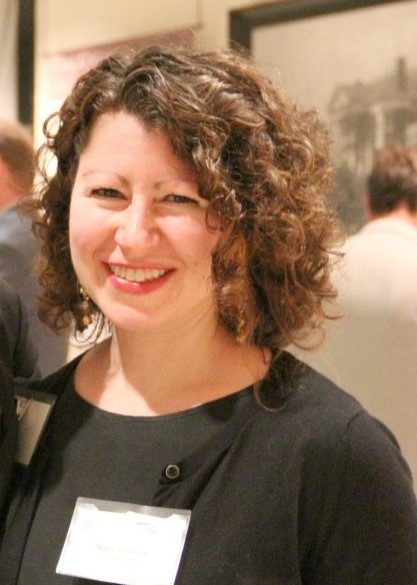
\includegraphics[scale=0.5]{mpsaraki.jpg}
    %\caption{}
    %\label{fig:my_label}
\end{figure}

I am in the master's program studying cybersecurity. I am currently in the process of a career transition; my previous job was as a Russian and French linguist. I am planning on graduating in May 2021, with the main goal of combining the skills I am getting now in this program in cybersecurity with the foreign languages I know.

In terms of research, I spent the summer doing the first three credits of my master's thesis, and I am looking to complete and defend it during this Fall semester. I am investigating the vulnerabilities of internet voting, comparing different implementations, and testing the code in one open-source implementation to see if it is in fact secure in terms of the security properties it claims to ensure.

To tell you a bit more about my background, I've lived in many different countries, mainly in Western Europe. I've had the opportunity to travel to Africa and Central Asia. I was also a "human test subject" at NASA, and tested exercise equipment that is now on the International Space Station.

Outside of my career pursuits, I am passionate about animal rescue, and have been a volunteer at the Humane Society for nearly five years.

Question (from Cassandra Putman): You went from learning different human languages to learning different programming languages.  Which one do you find more challenging to learn? 

%



\section{Introduction}
 \subsection{My Background}
My background has focused in mathematics and systems engineering.  Recently, I have decided to branch out into computer science and obtain a Master of Engineering in Cyber Security with an intent of focusing on hardware security.  I have a 17 year career in Department of Defense space systems including launch vehicles, space vehicles and most recently the ground systems that support the space vehicles.  System security, including software, hardware and physical security are of utmost importance to all the space programs I have worked, as they are often national security asset systems.
\subsection{My Research Interests and Course Goals}
I intend to focus my research in supply chain security with a focus on hardware security. While I'm fairly new to the computer science field and only recently started learning about blockchain, I do see a great utility and applicability being possible in applying blockchain technology to improve hardware supply chain security.  It appears, in my initial research, that applying blockchain technology to an IT supply chain, especially a supply chain that is as controlled as those that exist in government contracting, is both feasible and capable of providing great security benefits to the system, the user, and ultimately the security of the nation. I hope to narrow my research topic during this course and develop a focused and novel idea in the area of hardware supply chain security.
\subsection{My Personal Interests}
While I enjoy math and often read math related books, I also love to volunteer with a shar pei rescue.  I volunteer by performing temperament evaluations, transporting and fostering dogs and  performing home checks for potential fosters and adopters.  I have fostered 100+ dogs in the 12 years I have been volunteering with the shar pei rescue.  Beyond dog rescue, I also enjoy reading, hiking and doing crafts such as sewing and kitting. My love for travel has taken me to over 20 countries in the world, and I have plans to hit many more.  Figure 1 is a picture of me.
\begin{figure}[H]
    \centering
    \includegraphics[scale=0.5]{Images/cputman.jpg}
    \caption{Picture of Cassandra Putman}
    \label{fig:my_label}
\end{figure}







\section{Example of Easy Tables}
\csvautotabular{test.csv}


\section*{Better formated Tables}
    \begin{tabular}{r|r|r}%
    % specify table head    
    \bf Time (s) & \bf Rel. time (s)& \bf Y Pos
% use head of csv as column names
    \csvreader{test.csv}{}
% specify selected coloumns here    
    {\\\hline\csvcoli&\csvcolii&\csvcolvi}
    \end{tabular}
    \clearpage


\end{document}
